\documentclass[a4paper,12pt]{article}
\usepackage[latin1]{inputenc}
\usepackage[spanish]{babel}
\usepackage[dvips]{epsfig}
\usepackage{amsmath}
\usepackage{color}
\usepackage{graphicx}
\setlength{\textheight}{235mm}
\setlength{\textwidth}{168mm}
\setlength{\oddsidemargin}{0pt}
\pagestyle{empty}

\begin{document}
\mbox{}\vspace*{-45mm}

{\centering
{\small\sc Escuela T�cnica Superior de Ingenieros de Caminos, Canales y
Puertos (Madrid)}\\*[4mm]
{\Large\bf M�todo de los Elementos Finitos (2022-2023)}\\*[4mm]
PR�CTICA 9: Elementos estructurales: vigas \\*[4mm]
}

Se considera una viga en voladizo de secci�n rectangular de $1$ m de ancho, $1$ m de alto y  $L= 5$ m de longitud total. El material es el�stico lineal con propiedades mec�nicas
$E=27,0$ GPa y $\nu=0,3$. La viga est� empotrada en su extremo izquierdo y en su lado derecho se
aplica una carga puntual de 160 kN, tal como se indica en la figura.

\vspace{3mm}
Se pide realizar un modelo con elementos tipo viga lineales de {\em Timoshenko (B21)}. Discretizar para tener $6$ elementos. Adem�s, realizar modelos continuos con elementos tipo {\em plane stress}. Para estos �ltimos considerar lo siguiente:

\vspace{3mm}
\begin{enumerate}
	\item Malla de $1\times6$ elementos en el modelo, usar elementos tipo {\em CPS4, CPS4I, CPS4R y CPS8}
	\item Malla de $5\times26$ elementos en el modelo, usar elementos tipo {\em CPS4, CPS4I, y CPS8}
\end{enumerate}

\vspace{3mm}
El objetivo de la pr�ctica ser� comparar los resultados obtenidos con Abaqus con los arrojados por resistencia de materiales (ley de momentos flectores, de cortantes, reacciones en el empotramiento, flecha m�xima etc.) para el modelo con elementos tipo viga. Adem�s, analizar los valores de flechas m�ximas calculadas con los distintos tipos de modelo.

\begin{center}
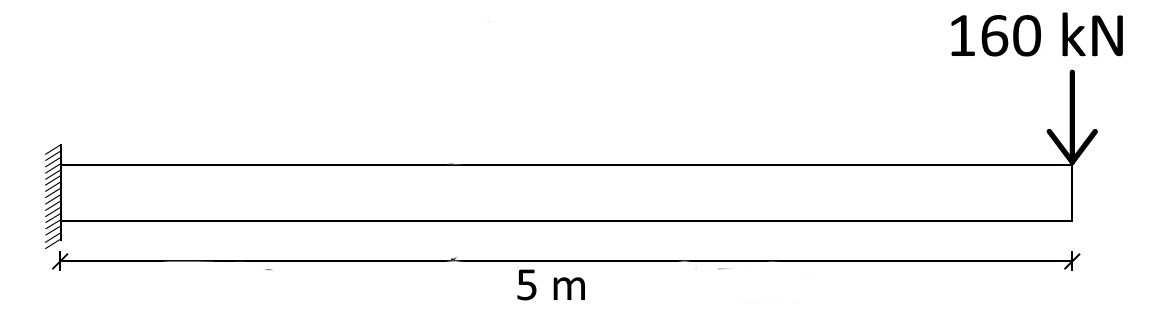
\includegraphics[width=0.7\textwidth]{figura}
\end{center}
%\noindent
\end{document}
